\documentclass[conference]{IEEEtran}
\usepackage{cite}
\usepackage{amsmath,amssymb,amsfonts}
\usepackage{algorithmic}
\usepackage{graphicx}
\usepackage{textcomp}
\usepackage{xcolor}
\usepackage{url}

\def\BibTeX{{\rm B\kern-.05em{\sc i\kern-.025em b}\kern-.08em
    T\kern-.1667em\lower.7ex\hbox{E}\kern-.125emX}}
\begin{document}

\title{
    Indor Robot Pose Estimation
}

\author{
    Eduardo Henrique Basilio de Carvalho
}

\maketitle

\begin{abstract}
    This report details the development and evaluation of algorithms for pose estimation of the Indor robot using laser and odometry data. We implemented and compared various filtering techniques, including the Unscented Kalman Filter, Extended Kalman Filter, and Particle Filter. Each method's performance was assessed based on accuracy and computational efficiency, with hyperparameter optimization conducted to enhance model performance. The findings underscore the significance of model selection in achieving effective pose filtering for the problem at hand.
\end{abstract}

\section{Introduction} \label{sec:introduction}

In the provided problem, the odometry data exhibits a noticeable drift, as discussed in Section \ref{sec:odometry}. This drift leads to a significant discrepancy between the odometry estimates and the reference data, which can adversely affect the overall pose estimation accuracy. While laser data has the potential to mitigate this drift by providing more accurate position information, it is important to note that laser readings are often subject to noise and other environmental factors. Consequently, relying solely on laser data for robot localization presents its own challenges. The integration of both odometry and laser data is essential for achieving a robust and reliable pose estimation, as it allows for the correction of odometry drift while leveraging the strengths of each data source.

Since the trajectory spans across several meters and the laser model exhibits dependency on the map structure, linear filtering approaches prove insufficient for achieving adequate pose estimates. The spatial variation of the environment introduces nonlinearities in the measurement model that cannot be adequately captured by linear filters such as the standard Kalman Filter. Consequently, nonlinear filtering techniques are necessary to properly account for these dynamics and provide reliable pose estimation \cite{Aguirre2007}. These advanced filtering methods are discussed in detail in Section \ref{sec:filters}.

\section{Map} \label{sec:map}

Figure \ref{fig:map} illustrates the environment in which the robotic experiments were conducted. The map is represented as a binary occupancy grid, where white pixels denote free space accessible to the robot, while black pixels represent obstacles and walls that must be avoided during navigation. This map representation is essential for the laser model, as it defines the expected measurement relationships between the robot's pose and the corresponding laser range observations.

\begin{figure}[htbp]
    \centerline{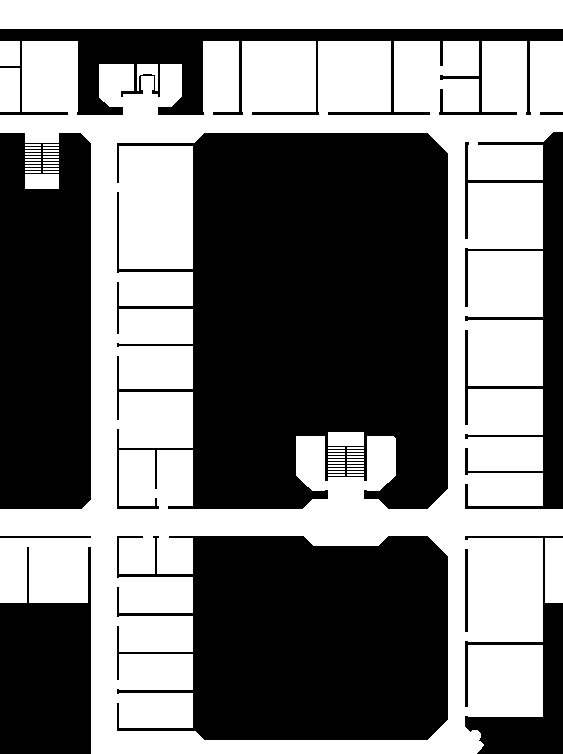
\includegraphics[width=\linewidth]{map.png}}
    \caption{Map of the environment where the Indor robot operates.}
    \label{fig:map}
\end{figure}

\subsection{Transformation to Data's Frame} \label{sec:transformation_to_data_frame}

The source material provides the map in conventional coordinates with pixel-scale representation. However, since the experimental data is provided in a shifted, rotated, and scaled reference frame, several coordinate transformations were necessary to ensure consistency between the map and the data. The following transformations were applied in sequence:

\begin{enumerate}
    \item \textbf{Origin Centering:} The coordinate system was translated such that the origin $(0, 0)$ is positioned at the center of the map, rather than at a corner. This transformation is defined as:
    \begin{equation}
        x' = x - \frac{w}{2}, \quad y' = y - \frac{h}{2}
    \end{equation}
    where $w$ and $h$ are the width and height of the map in pixels, respectively.
    
    \item \textbf{Y-axis Inversion:} The $y$-axis was inverted to align with the data's coordinate convention, transforming the pixel coordinates from image space to a standard Cartesian frame:
    \begin{equation}
        y'' = -y'
    \end{equation}
    
    \item \textbf{Scale Conversion:} Pixel coordinates were converted to metric units using the provided scale factor $s$ (in meters per pixel):
    \begin{equation}
        x_m = s \cdot x', \quad y_m = s \cdot y''
    \end{equation}
    
    \item \textbf{Spatial Cropping:} The map was cropped to focus on the region of interest encompassing the experimental trajectory, reducing computational overhead while maintaining the necessary environmental context for laser-based localization.
\end{enumerate}

These transformations ensure that the map representation is consistent with the odometry and laser data frames, enabling accurate pose estimation throughout the experiment.

\section{Data} \label{sec:data}

The experimental data was initially provided in a single space-separated file, which contained various measurements and observations relevant to the pose estimation task. To enhance organization and facilitate subsequent processing, this data was systematically divided into three distinct comma-separated files. Each file corresponds to a specific type of data: reference data, laser measurements, and odometry readings.

This separation allows for more efficient data handling and processing, as each file can be independently accessed and manipulated according to its specific requirements. The reference data file contains the ground truth positions against which the estimated poses can be compared. The laser measurements file includes the range and bearing information captured by the robot's laser sensors, while the odometry readings file records the robot's estimated position based on its movement and wheel encoders.

If we denote the original data as \( D \) and the separated files as \( D_{ref} \), \( D_{laser} \), and \( D_{odom} \), we can express the separation process as follows:

\[
D = \{D_{ref}, D_{laser}, D_{odom}\}
\]

This structured approach not only improves clarity but also streamlines the data preprocessing steps that follow, ensuring that each dataset can be effectively utilized in the filtering and estimation algorithms discussed in subsequent sections.

\subsection{Reference} \label{sec:reference}

The reference data is provided in the global frame with absolute values, which is crucial for accurate pose estimation. This dataset consists of three columns: the first column contains the \( x \) coordinates, representing the robot's position along the horizontal axis; the second column contains the \( y \) positions, indicating the robot's position along the vertical axis; and the third column contains the yaw angles, denoted as \( \theta \), which represent the orientation of the robot in radians.

Mathematically, we can express the reference data as a set of tuples \( R \) defined as follows:

\[
R = \{(x_i, y_i, \theta_i) \mid i = 1, 2, \ldots, N\}
\]

where \( N \) is the total number of observations. Each tuple \( (x_i, y_i, \theta_i) \) corresponds to a specific time step \( i \) and provides essential information for evaluating the performance of the pose estimation algorithms. The yaw angle \( \theta_i \) is particularly important as it allows for the transformation of the robot's pose from the global frame to the local frame, facilitating the integration of laser and odometry data in subsequent filtering processes.

\begin{figure}[htbp]
    \centerline{
\includegraphics[width=\linewidth]{reference_trajectory.png}}
    \caption{Reference trajectory of the Indor robot in the global frame.}
    \label{fig:reference_trajectory}
\end{figure}

Figure \ref{fig:reference_trajectory} presents a visual representation of the reference data plotted over the map of the environment. This overlay allows for a direct comparison between the estimated poses derived from the filtering algorithms and the ground truth positions provided in the reference dataset. 

Mathematically, we can denote the reference positions as \( R = \{(x_i, y_i, \theta_i) \mid i = 1, 2, \ldots, N\} \), where each tuple corresponds to the robot's position and orientation at discrete time steps. The plotted reference trajectory serves as a benchmark for evaluating the accuracy of the pose estimation methods employed in this study.

The visualization not only highlights the trajectory of the Indor robot but also emphasizes the spatial relationship between the robot's estimated poses and the obstacles present in the environment. This context is crucial for understanding the performance of the filtering techniques, as it illustrates how well the algorithms navigate through the mapped space while adhering to the constraints imposed by the environment.

In the subsequent sections, we will analyze the discrepancies between the reference data and the estimated poses, providing insights into the effectiveness of the various filtering approaches utilized in this research.

\subsection{Laser} \label{sec:laser}

The laser data comprises 360 columns, each corresponding to a single laser sensor reading. These sensors are angularly displaced by 0.5 degrees from one another, collectively covering the 180-degree frontal hemisphere of the robot. Mathematically, the angular coverage can be expressed as:

\begin{equation}
    \Delta\phi = 0.5\deg, \quad \Phi_{total} = 360 \times 0.5\deg = 180\deg
\end{equation}

where $\Delta\phi$ denotes the angular separation between adjacent sensors and $\Phi_{total}$ represents the total angular coverage.

Each sensor returns a range measurement in meters, representing the distance to the nearest obstacle detected in its corresponding direction. These measurements are expected to fall within the range $[0, 8]$ meters, defining the operational range of the laser scanner. The laser data can be represented as a vector of measurements $L$ at each time step:

\[
L = \{r_j \mid r_j \in [0, 8] \text{ m}, \quad j = 1, 2, \ldots, 360\}
\]

where $r_j$ denotes the range reading from the $j$-th sensor. This rich angular resolution provides detailed geometric information about the robot's surroundings, which is essential for accurate position correction in the pose estimation algorithms discussed in Section \ref{sec:laser_model}.

\begin{figure}[htbp]
    \centerline{
\includegraphics[width=\linewidth]{laser_scan.png}}
    \caption{Laser scan at a specific time step. Each red dot corresponds to a laser measurement.}
    \label{fig:laser_scan}
\end{figure}

Figure \ref{fig:laser_scan} illustrates a sample laser scan taken at a specific time step. In this figure, each red dot represents a laser measurement projected into the environment based on the robot's current pose. The distribution of these measurements provides insight into the spatial configuration of obstacles around the robot, which is crucial for effective localization and navigation.

In the context of the robot's pose and laser range data, we can express the transformation of laser readings into global Cartesian coordinates mathematically. 

Let:

\begin{itemize}
    \item \( (x, y, \theta) \) represent the robot's position and orientation, where \( x \) and \( y \) are the coordinates in the global frame, and \( \theta \) is the heading angle.
    \item \( r_i \) denote the laser range measurement at angle \( \alpha_i \) relative to the robot's heading.
\end{itemize}

The global coordinates of the laser points can be computed as follows:

\begin{enumerate}
    \item For each laser reading, the global angle is given by:
    
    \begin{equation}
        \text{global\_angle}_i = \theta + \alpha_i
    \end{equation}

\item The Cartesian coordinates of the laser point in the global frame are then calculated using:

   \begin{align*}
   x_{\text{laser}, i} & = x + r_i \cdot \cos(\text{global\_angle}_i) \\
   y_{\text{laser}, i} & = y + r_i \cdot \sin(\text{global\_angle}_i)
   \end{align*}
\end{enumerate}

This transformation ensures that the laser readings, which are initially in polar coordinates relative to the robot's local frame, are accurately represented in the global Cartesian coordinate system. The filtering condition \( 0.1 < r_i < 8.0 \) ensures that only valid laser readings are considered for this transformation.

\subsection{Odometry} \label{sec:odometry}

The odometry data serves as a crucial component in understanding the robot's movement throughout the experiment. It provides the cumulative displacement of the robot from its initial pose, allowing for the assessment of its trajectory over time. Each row in the odometry dataset corresponds to the global displacement from the starting position to a specific moment in the experiment.

Mathematically, we can represent the odometry data as a set of tuples \( O \) defined as follows:

\[
O = \{(x_i, y_i, \theta_i) \mid i = 1, 2, \ldots, N\}
\]

where \( N \) is the total number of observations. In this representation, the first column contains the \( x \) coordinates, indicating the robot's position along the horizontal axis; the second column contains the \( y \) coordinates, representing the robot's position along the vertical axis; and the third column contains the yaw angles, denoted as \( \theta \), which indicate the orientation of the robot in radians.

The cumulative displacement can be expressed as:

\[
\Delta x = x_i - x_0, \quad \Delta y = y_i - y_0, \quad \Delta \theta = \theta_i - \theta_0
\]

where \( (x_0, y_0, \theta_0) \) represents the initial pose of the robot. This formulation allows for the calculation of the robot's position and orientation at any given time step \( i \) relative to its starting point.

It is important to note that the odometry data serves as the input to the odometry models discussed in Section \ref{sec:odometry_model}. Rather than providing a reference for evaluation, the odometry model functions as the \textit{process model} \cite{Aguirre2007} in the estimation techniques employed in this work. Specifically, the odometry model generates predictions of the robot's pose evolution that are subsequently corrected by the integration of laser measurements through the filtering algorithms. The predictions from the odometry model are refined by the filtering techniques to account for the accumulated drift and produce more accurate pose estimates. This correction mechanism is central to the effectiveness of the Unscented Kalman Filter, Extended Kalman Filter, and Particle Filter approaches discussed in Section \ref{sec:filters}.

\section{Data Preprocessing} \label{sec:data_preprocessing}

Before the main problem of pose estimation is addressed, the experimental data must undergo preprocessing to facilitate subsequent identification and filtering operations. The preprocessing steps are designed to extract a representative subset of the data that captures the essential dynamics of the robotic experiment while reducing computational burden. Formally, if we denote the complete dataset as $D = \{D_{ref}, D_{laser}, D_{odom}\}$ with $N$ total observations, the preprocessing aims to produce a reduced dataset $D' \subset D$ with $N' < N$ observations such that:

\begin{equation}
    \mathcal{C}(D') \ll \mathcal{C}(D)
\end{equation}

where $\mathcal{C}(\cdot)$ represents the computational cost of subsequent filtering and estimation operations, while maintaining sufficient fidelity to the original experimental characteristics.

The preprocessing strategy employed in this work comprises two main steps: data decimation, which reduces the sampling frequency to achieve computational efficiency, and trajectory trimming, which removes the initial and final segments of the trajectory that may contain noise or irrelevant movements. These operations are described in detail in the following subsections.

\subsection{Decimation} \label{sec:decimation}

Data decimation is performed to reduce the computational burden of subsequent filtering operations while preserving the essential dynamics of the robot's trajectory \cite{Aguirre2007}. The decimation process selects a subset of the original observations at regular intervals, effectively reducing the sampling frequency. If the original dataset contains $N$ observations sampled at frequency $f_s$, decimation with factor $d$ yields a reduced dataset with $N' = \lfloor N / d \rfloor$ observations sampled at frequency $f_s' = f_s / d$.

The decimation factor was determined through a systematic trial-and-error manual process. Various decimation ratios were tested by applying each factor to the complete dataset and subsequently visualizing the resulting reference trajectory overlaid on the environment map. This visual inspection approach allowed for qualitative assessment of how well the decimated trajectory preserved the essential characteristics of the original path. The selection criterion was to identify the highest decimation factor that yielded a trajectory sufficiently similar to the original, thereby minimizing data while maintaining fidelity to the experimental dynamics.

Following this evaluation procedure, a decimation factor of $d = 100$ was selected as the optimal compromise between computational efficiency and trajectory preservation. This factor reduces the dataset by two orders of magnitude, substantially decreasing the computational requirements for the filtering algorithms discussed in Section \ref{sec:filters}, while ensuring that the decimated trajectory adequately represents the robot's movement through the environment.

It is important to note that all figures and results presented throughout this document already reflect the application of this decimation factor. Consequently, the visualizations and quantitative analyses shown hereafter correspond to the reduced dataset with sampling frequency $f_s' = f_s / 100$.

\subsection{Trimming} \label{sec:trimming}

Trajectory trimming is performed to eliminate segments of the robot's path that may introduce noise or irrelevant movements, particularly at the beginning and end of the experiment. These segments often contain transient behaviors, such as manual positioning or stopping maneuvers, which do not contribute meaningfully to the analysis of the robot's steady-state navigation performance. By removing these portions of the trajectory, the focus is placed on the segments where the robot is actively navigating the environment, thereby enhancing the quality of the data used for filtering and estimation. The first 10 and last 50 observations were removed from the dataset, resulting in a trimmed trajectory that better represents the robot's operational behavior during the experiment.

\section{Laser Model} \label{sec:laser_model}

\subsection{Linear Dynamic Model} \label{sec:laser_model_linear}

The laser-based position estimation task is formulated as a discrete-time linear dynamic system where the robot's state evolves according to laser measurements. The state vector comprises three components: horizontal position, vertical position, and orientation angle. At each time step, the state transition is governed by a linear relationship between the current state, extracted laser features, and a bias term.

Formally, the model is defined as:

\begin{equation}
    \mathbf{x}_{k+1} = \mathbf{A} \mathbf{x}_k + \mathbf{B} \mathbf{f}(\mathbf{s}_k) + \mathbf{b}
\end{equation}

where:
\begin{itemize}
    \item $\mathbf{x}_k = [x_k, y_k, \theta_k]^T$ is the state vector at time step $k$
    \item $\mathbf{A} \in \mathbb{R}^{3 \times 3}$ is the state transition matrix
    \item $\mathbf{f}(\mathbf{s}_k) \in \mathbb{R}^6$ is a feature vector extracted from the laser scan
    \item $\mathbf{B} \in \mathbb{R}^{3 \times 6}$ is the laser feature weight matrix
    \item $\mathbf{b} \in \mathbb{R}^3$ is a bias vector
\end{itemize}

\subsubsection{Laser Feature Extraction}

Rather than using all 360 laser measurements directly, six summary statistics are computed to reduce dimensionality while capturing essential geometric information about the robot's surroundings. These features are:

\begin{equation}
    \mathbf{f}(\mathbf{s}) = [\mu, r_{\min}, \sigma, \mu_{\text{left}}, \mu_{\text{front}}, \mu_{\text{right}}]^T
\end{equation}

where:
\begin{itemize}
    \item $\mu = \frac{1}{360}\sum_{j=1}^{360} r_j$ is the mean of all laser ranges
    \item $r_{\min} = \min(r_1, r_2, \ldots, r_{360})$ is the minimum range (closest obstacle)
    \item $\sigma = \sqrt{\frac{1}{360}\sum_{j=1}^{360}(r_j - \mu)^2}$ is the standard deviation
    \item $\mu_{\text{left}}, \mu_{\text{front}}, \mu_{\text{right}}$ are mean ranges computed over the left (sensors 1--120), front (sensors 121--240), and right (sensors 241--360) sectors respectively
\end{itemize}

These features capture both global context (mean, minimum, standard deviation) and local directional information about the environment relative to the robot's heading.

\subsubsection{Model Identification}

The model parameters $\{\mathbf{A}, \mathbf{B}, \mathbf{b}\}$ are identified from experimental data using linear regression \cite{Aguirre2007}. Given reference trajectory data $\{\mathbf{x}_0, \mathbf{x}_1, \ldots, \mathbf{x}_N\}$ and corresponding laser scans $\{\mathbf{s}_0, \mathbf{s}_1, \ldots, \mathbf{s}_N\}$, the regression problem is formulated as:

\begin{equation}
    \min_{\mathbf{A}, \mathbf{B}, \mathbf{b}} \sum_{k=0}^{N-\Delta} \left\| \mathbf{x}_{k+\Delta} - (\mathbf{A} \mathbf{x}_k + \mathbf{B} \mathbf{f}(\mathbf{s}_k) + \mathbf{b}) \right\|_2^2
\end{equation}

where $\Delta$ is a time step parameter (typically $\Delta = 1$). This optimization problem is solved using ordinary least squares regression, yielding closed-form solutions for the model parameters.

\subsection{Nonlinear AutoRegressive eXogenous (NARX) Model} \label{sec:laser_model_narx}

To capture nonlinear relationships between laser observations and state evolution, a NARX model is employed \cite{scikit-learn}. This approach incorporates past state information through an autoregressive structure, allowing the model to learn temporal dependencies in the robot's dynamics.

The NARX model is defined as:

\begin{equation}
    \mathbf{x}_{k+1} = g(\mathbf{x}_k, \mathbf{x}_{k-1}, \ldots, \mathbf{x}_{k-n_{\text{lag}}+1}, \mathbf{f}(\mathbf{s}_k))
\end{equation}

where $g(\cdot)$ is a nonlinear function parameterized by a machine learning model, and $n_{\text{lag}}$ is the number of past time steps (lags) used as autoregressive inputs.

The input feature vector concatenates past state history and current laser features:

\begin{equation}
    \mathbf{u}_k = [\mathbf{x}_k, \mathbf{x}_{k-1}, \ldots, \mathbf{x}_{k-n_{\text{lag}}+1}, \mathbf{f}(\mathbf{s}_k)]^T
\end{equation}

Three model variants are investigated:

\begin{enumerate}
    \item \textbf{Linear NARX:} A ridge regression model with $\ell_2$ regularization applied directly to the augmented feature vector.
    
    \item \textbf{Polynomial NARX:} Ridge regression applied to polynomial expansions of the input features, capturing nonlinear interactions up to a specified degree.
    
    \item \textbf{Neural NARX:} A multilayer perceptron with rectified linear activation functions, trained via stochastic gradient descent with early stopping to prevent overfitting.
\end{enumerate}

\subsubsection{Hyperparameter Optimization}

Given the number of potential hyperparameters, a systematic grid search with time series cross-validation is performed to identify optimal configurations. The search space includes:

\begin{itemize}
    \item Number of lags: $n_{\text{lag}} \in \{2, 3, 5\}$
    \item Model type: $\{\text{linear}, \text{polynomial}, \text{neural}\}$
    \item Polynomial degree (if applicable): $\{2, 3\}$
    \item Neural network hidden layer configurations (if applicable)
    \item Regularization strength: $\alpha \in \{0.001, 0.01, 0.1\}$
\end{itemize}

Time series cross-validation is employed rather than random cross-validation to respect the temporal structure of the data \cite{scikit-learn}. The dataset is divided into sequential folds, where earlier data is used for training and subsequent data for validation, preventing information leakage from future to past observations.

\subsubsection{Selected Model}

Based on grid search results, the optimal configuration exhibits the following characteristics: a linear NARX model with two lags, ridge regularization strength of 0.01, utilizing input features from both past and present time steps. This configuration achieves root mean square error values of approximately $[0.128, 0.077, 0.808]$ meters per state component (horizontal position, vertical position, and orientation) on the validation dataset.

The selection of a linear model over nonlinear variants suggests that the relationship between laser features and state evolution is primarily linear within the operational regime studied. The modest input dimensionality ($2 \times 3 + 6 = 12$ features) and the strong performance without polynomial expansion or neural network complexity indicate that the essential predictive information is captured by the linear relationships encoded in the model coefficients.

\begin{figure}[htbp]
    \centerline{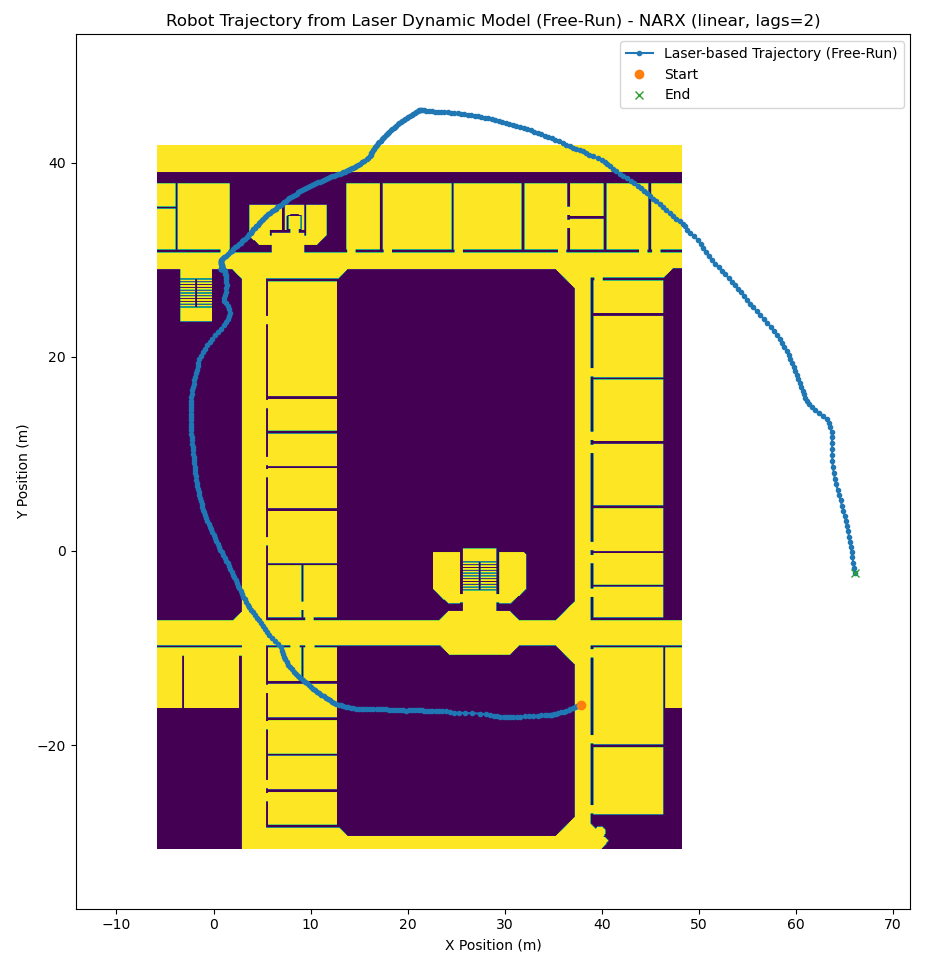
\includegraphics[width=\linewidth]{laser_model_freerun.png}}
    \caption{Free-run simulation of the laser model.}
    \label{fig:laser_model_freerun}
\end{figure}

\begin{figure}[htbp]
    \centerline{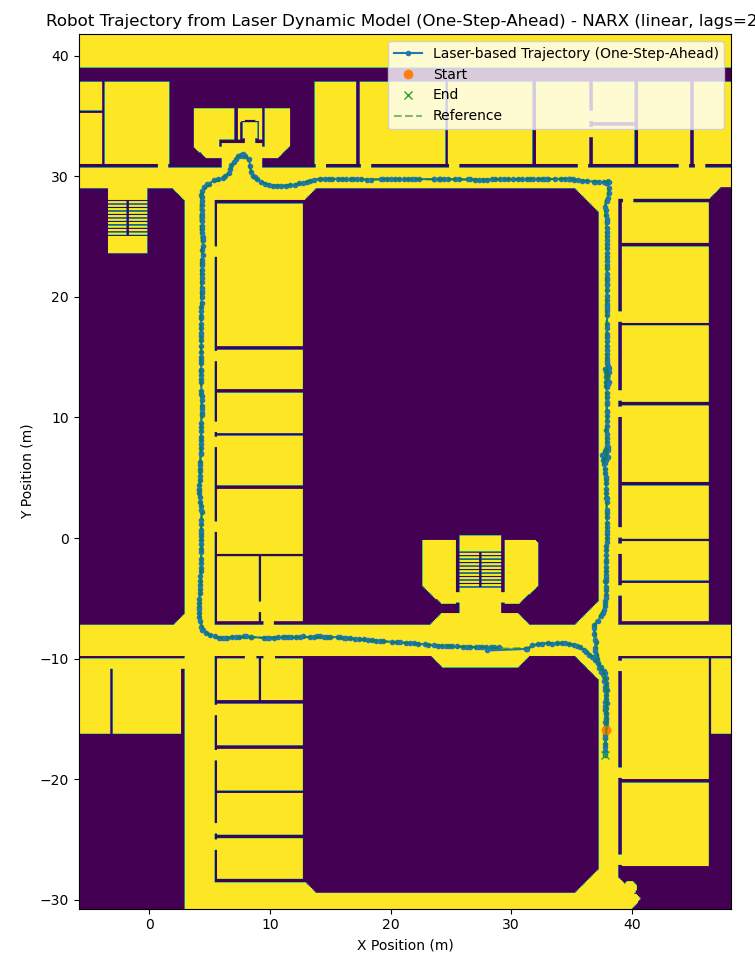
\includegraphics[width=\linewidth]{laser_model_onestep.png}}
    \caption{One-step ahead simulation of the laser model.}
    \label{fig:laser_model_onestep}
\end{figure}

The validation of the laser model reveals important insights into its predictive capabilities and limitations. Figure \ref{fig:laser_model_freerun} presents a free-run simulation where the model operates autonomously, using only its own predictions as input for subsequent time steps. Starting from the initial reference pose $\mathbf{x}_0$, the model generates predictions iteratively according to:

\begin{equation}
    \hat{\mathbf{x}}_{k+1} = \mathbf{A} \hat{\mathbf{x}}_k + \mathbf{B} \mathbf{f}(\mathbf{s}_k) + \mathbf{b}
\end{equation}

where $\hat{\mathbf{x}}_k$ denotes the model's own prediction at time step $k$. While this autonomous simulation succeeds in capturing the general trajectory morphology, it exhibits severe degradation in precision. The accumulated prediction errors compound over time, resulting in substantial deviations from the reference trajectory and rendering the free-run simulation unsuitable for direct pose estimation applications. The root mean square error grows progressively with prediction horizon, illustrating the accumulation of modeling uncertainty.

In contrast, Figure \ref{fig:laser_model_onestep} demonstrates the performance of one-step ahead prediction, where the model receives the true state at each time step and predicts only the immediate next state:

\begin{equation}
    \hat{\mathbf{x}}_{k+1} = \mathbf{A} \mathbf{x}_k + \mathbf{B} \mathbf{f}(\mathbf{s}_k) + \mathbf{b}
\end{equation}

This one-step prediction exhibits markedly superior performance, with estimates closely tracking the reference trajectory throughout the experiment. The laser model achieves high fidelity when operating with access to ground truth state information, suggesting that the model has learned accurate local dynamics and that prediction errors primarily arise from accumulated drift rather than fundamental model inadequacy. This characteristic makes the laser model particularly well-suited as a measurement update component within filtering frameworks, where the filtering algorithms can provide corrected state estimates at each time step, thereby preventing error accumulation. The high one-step prediction accuracy validates the model's suitability for integration into the Unscented Kalman Filter, Extended Kalman Filter, and Particle Filter approaches discussed in Section \ref{sec:filters}.

\section{Odometry Model} \label{sec:odometry_model}

\subsection{Original Odometry Model} \label{sec:odometry_model_original}

The odometry data, as detailed in Section \ref{sec:odometry}, is provided in the global reference frame with measurements expressed as cumulative displacements from the robot's initial pose. Given this characteristic, the original and most straightforward odometry model employs a static assumption wherein the robot's pose at any time step $k$ is computed by simply adding the odometry displacement to the initial pose.

Formally, let $\mathbf{x}_0 = [x_0, y_0, \theta_0]^T$ denote the initial pose of the robot and $\mathbf{o}_k = [\Delta x_k, \Delta y_k, \Delta \theta_k]^T$ represent the cumulative odometry displacement at time step $k$. The original odometry model is then defined as:

\begin{equation}
    \mathbf{x}_k = \mathbf{x}_0 + \mathbf{o}_k
\end{equation}

This linear, time-invariant model assumes that the odometry measurements accurately reflect the robot's true displacements without drift or systematic errors. In practice, however, odometry data accumulated over extended trajectories typically exhibits significant drift, as the errors in wheel encoders and other motion sensors compound over time. As discussed in Section \ref{sec:introduction}, this drift manifests as an increasing discrepancy between the odometry-based estimates and the ground truth reference data, particularly over the several meters spanned by the experimental trajectory.

Despite its simplicity, this static model serves as a baseline for understanding the limitations of odometry-based localization and motivates the necessity of integrating laser measurements through advanced filtering techniques. The comparison between this original model's predictions and the reference data quantifies the magnitude of odometry drift and establishes the performance gap that the filtering algorithms aim to bridge through sensor fusion.

\begin{figure}[htbp]
    \centerline{
\includegraphics[width=\linewidth]{original_odo_model.png}}
    \caption{Original odometry model free-run simulation.}
    \label{fig:original_odo_model}
\end{figure}

Figure \ref{fig:original_odo_model} demonstrates that the original static odometry model captures local movements of the robot with notable precision over short time intervals. However, the model exhibits pronounced drift when operated in free-run mode over the complete experimental trajectory. This drift accumulates progressively, resulting in substantial deviations from the reference trajectory as the mission duration extends. The root cause of this degradation lies in the inherent limitations of odometry-based localization: incremental errors from wheel encoders and inertial sensors compound over time, leading to systematic bias in the estimated pose.

Given that the odometry model serves as the \textit{process model} in the filtering framework, as discussed in Section \ref{sec:odometry_model}, the fidelity of odometry predictions directly influences the quality of the filtering estimates. A more accurate process model would reduce the prediction uncertainty and allow the filtering algorithms to operate more effectively within their respective correction mechanisms. This observation motivates the development of an improved odometry model that better captures the dynamics of robot motion and mitigates accumulated drift.

Despite the limitations of the original odometry model, an important insight emerges from the joint consideration of the odometry and laser models: even a modestly accurate laser model can effectively correct smaller pose mismatches introduced by odometry drift. The laser model, when integrated into a filtering framework, provides measurement updates that anchor the robot's estimated pose to environmental features encoded in the map. Since the laser measurements contain rich geometric information about the robot's surroundings, they can resolve ambiguities in the pose estimate that arise from odometry errors. Consequently, the combination of a corrected process model and laser-based measurement updates through advanced filtering techniques represents a promising approach for robust pose estimation, even when individual models exhibit limitations.

\subsection{Odometry Data Differentiation} \label{sec:odometry_model_differentiation}

To enhance the odometry model's fidelity and better capture the robot's motion dynamics, the cumulative odometry data is transformed into incremental displacements between consecutive time steps. This differentiation process allows the model to represent the robot's movement as a series of small, discrete steps rather than a single cumulative displacement from the initial pose. Formally, let $\mathbf{o}_k = [\Delta x_k, \Delta y_k, \Delta \theta_k]^T$ denote the cumulative odometry displacement at time step $k$. The incremental odometry displacement $\Delta \mathbf{o}_k$ between time steps $k-1$ and $k$ is computed as:

\begin{equation}
    \begin{aligned}
        \Delta \mathbf{o}_k &= \mathbf{o}_k - \mathbf{o}_{k-1} \\
                            &= [\Delta x_k - \Delta x_{k-1}, \Delta y_k - \Delta y_{k-1}, \Delta \theta_k - \Delta \theta_{k-1}]^T
    \end{aligned}
\end{equation}

This transformation yields a sequence of incremental displacements $\{\Delta \mathbf{o}_1, \Delta \mathbf{o}_2, \ldots, \Delta \mathbf{o}_N\}$ that more accurately reflects the robot's motion dynamics over time. By modeling the robot's pose evolution as a series of small steps, the odometry model can better account for variations in speed, direction changes, and other dynamic factors that influence the robot's trajectory.

\subsection{Model Selection and Parameter Estimation} \label{sec:odometry_model_selection}

Similar to the laser model identification process described in Section \ref{sec:laser_model_narx}, the odometry model was estimated through a systematic grid search with time series cross-validation to identify optimal hyperparameters. Given the temporal structure of odometry data and the need to prevent information leakage, the same cross-validation strategy employed for laser model selection was applied to the odometry model development.

The odometry model identification process follows an analogous structure to the laser model, wherein incremental odometry displacements $\{\Delta \mathbf{o}_1, \Delta \mathbf{o}_2, \ldots, \Delta \mathbf{o}_N\}$ serve as inputs to predict subsequent state changes. A NARX architecture was selected for the odometry model, incorporating past state information through an autoregressive structure defined as:

\begin{equation}
    \Delta \mathbf{x}_{k+1} = h(\mathbf{x}_k, \mathbf{x}_{k-1}, \ldots, \mathbf{x}_{k-n_{\text{lag}}+1}, \Delta \mathbf{o}_k)
\end{equation}

where $h(\cdot)$ is a function parameterized by a machine learning model, and $n_{\text{lag}}$ denotes the number of past time steps incorporated into the model.

The hyperparameter search space encompassed:

\begin{itemize}
    \item Number of lags: $n_{\text{lag}} \in \{1, 2, 3, 5\}$
    \item Model type: $\{\text{linear}, \text{polynomial}, \text{neural}\}$
    \item Polynomial degree (if applicable): $\{2, 3\}$
    \item Neural network hidden layer configurations (if applicable)
    \item Regularization strength: $\alpha \in \{0.001, 0.01, 0.1, 1.0\}$
\end{itemize}

The optimal odometry model configuration, identified through exhaustive grid search, exhibits the following characteristics: a linear NARX model with a single lag ($n_{\text{lag}} = 1$), employing ridge regularization with strength $\alpha = 0.2$ and $n_{\text{features}} = 6$ input dimensions. This configuration achieves root mean square error values of $[0.127, 0.081, 0.820]$ meters per state component (horizontal position, vertical position, and orientation angle) on the validation dataset. The complete model specification and performance metrics are documented in the model configuration file.

The selection of a linear NARX model for odometry, consistent with the laser model selection, indicates that the relationship between incremental odometry measurements and state evolution is predominantly linear within the operational domain. The parsimonious architecture ($n_{\text{lag}} = 1$) suggests that short-term temporal dependencies dominate the odometry dynamics, and that incorporating information from multiple past lags does not substantially improve predictive performance while increasing model complexity.

\begin{figure}[htbp]
    \centerline{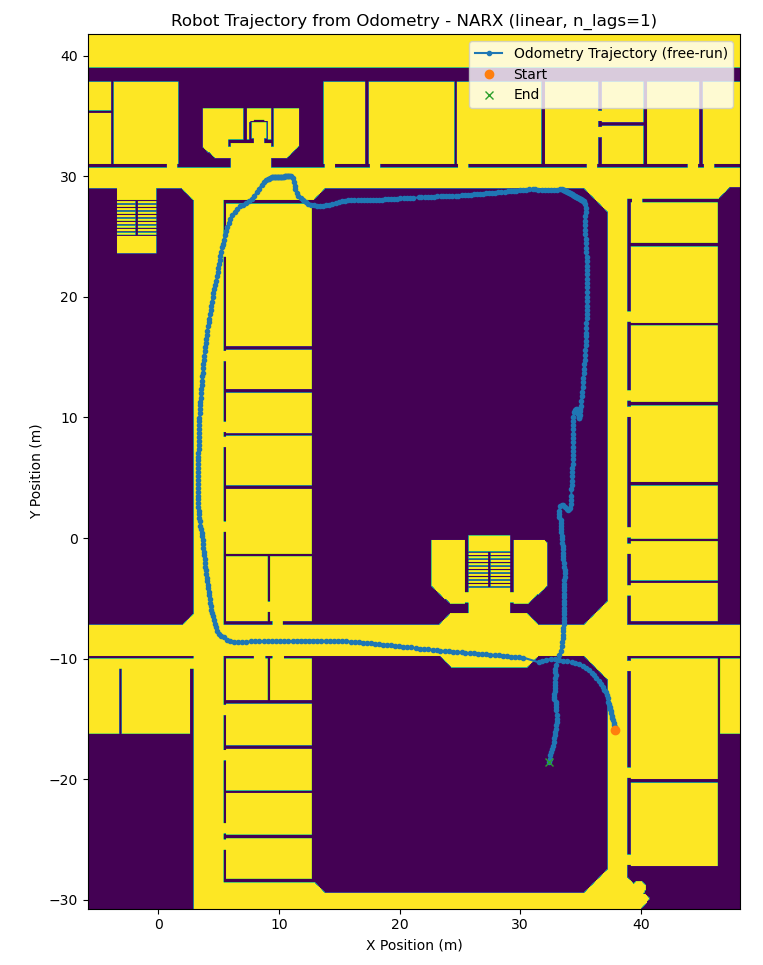
\includegraphics[width=\linewidth]{odo_model_freerun.png}}
    \caption{Free-run simulation of the odometry model.}
    \label{fig:odo_model_freerun}
\end{figure}

Figure \ref{fig:odo_model_freerun} reveals that the identified odometry model substantially improves upon the original static model, demonstrating markedly superior global trajectory fidelity throughout the experimental duration. While the identified model exhibits slightly reduced local precision in capturing fine-grained movements between consecutive time steps compared to the original cumulative model, this trade-off yields significant advantages in global consistency. The identified model's trajectory remains coherent and continuous over the complete mission duration, whereas the original model's accumulated drift causes progressive divergence from the reference path.

Quantitatively, the improvement manifests in the reduced systematic bias accumulation over extended prediction horizons. The identified linear NARX odometry model, with its learned parameters optimized through time series cross-validation, captures the underlying dynamics of robot motion more accurately than the static assumption. This enhanced process model, when integrated into the filtering framework discussed in Section \ref{sec:filters}, provides superior predictions upon which the filtering algorithms can base their correction mechanisms.

However, despite these improvements, the odometry model alone remains insufficient for achieving high-fidelity pose estimation. The free-run simulation still exhibits noticeable deviations from the reference trajectory, particularly in regions where the robot navigates complex environmental geometry. This residual error underscores the fundamental limitation of odometry-based localization: even with sophisticated learned dynamics models, incremental sensor errors inevitably compound over extended trajectories. The integration of laser-based measurement updates through the advanced filtering techniques is therefore essential to anchor the pose estimates to environmental features and provide the final correction necessary for accurate and robust robot localization.

The comparison between Figures \ref{fig:original_odo_model} and \ref{fig:odo_model_freerun} thus illustrates the complementary roles of improved process models and measurement-based filtering in achieving reliable pose estimation. The identified odometry model substantially reduces the prediction uncertainty that filtering algorithms must overcome, thereby enhancing the overall effectiveness of the complete estimation system.

\section{Filters} \label{sec:filters}

This section introduces the three filtering algorithms employed for robot pose estimation: the Unscented Kalman Filter (UKF), Extended Kalman Filter (EKF), and Particle Filter (PF). All three methods address the fundamental challenge of fusing noisy odometry and laser measurements to produce robust pose estimates.

\subsubsection{Common Framework}

Despite their algorithmic differences, all three filters share a unified architecture comprising predict and update steps operating on a common state representation. The state vector $\mathbf{x}_k = [x_k, y_k, \theta_k]^T$ remains constant across implementations, along with process noise covariance $\mathbf{Q}$ and measurement noise covariance $\mathbf{R}$, both parameterized by standard deviation tuples $(q_{std}, r_{std})$.

A key architectural commonality is the integration of dual one-step-ahead models: the odometry model (Section \ref{sec:odometry_model}) serves as the process model generating control predictions, while the laser model (Section \ref{sec:laser_model}) generates measurement predictions. Both models are reset to the current fused state estimate at each iteration, preventing error accumulation and enabling the filters to operate effectively despite the nonlinearities present in the laser measurement model.

\subsubsection{Initialization and Hyperparameter Tuning}

All three filters are initialized identically with the robot's initial pose and diagonal covariance matrices reflecting confidence in the initial state estimate. Hyperparameters including noise standard deviations and, for the Particle Filter, the number of particles and resampling threshold, are loaded from tuned parameter files with fallback to default values. This parameterization enables systematic hyperparameter optimization across all filters using a common protocol.

\subsubsection{Model Integration}

Each filter accommodates both linear and NARX laser models through a unified loading interface. The selection between model types is transparent to the filtering algorithm, allowing the same filter implementation to operate with different underlying dynamic models. Similarly, optional NARX odometry models are supported, with fallback to a simple additive odometry model when no specialized model is provided.

\subsubsection{Similarities and Differences}

The predict step is semantically equivalent across all three methods: the odometry model generates a one-step-ahead prediction from the current state, producing a control delta that is applied with process noise. The update step, however, differs substantially. The EKF and UKF employ principled covariance-based update mechanisms (exploiting Jacobians and sigma points respectively), whereas the Particle Filter implements likelihood-weighted resampling to redistribute particle mass according to measurement fit.

The output of all three filters is an array of sequential state estimates, which are visualized identically against the odometry baseline and environment map, facilitating direct algorithmic comparison.

\subsection{Unscented Kalman Filter} \label{sec:unscented_kalman_filter}

The Unscented Kalman Filter (UKF) is a nonlinear filtering technique that extends the principles of Kalman filtering to systems with significant nonlinearities \cite{Aguirre2007}. Unlike the Extended Kalman Filter, which linearizes the system dynamics around the current state estimate through Jacobian computation, the UKF employs a deterministic sampling strategy to propagate probability distributions through nonlinear transformations while preserving mean and covariance statistics.

\subsubsection{Theoretical Foundation}

The fundamental advantage of the UKF over linearization-based approaches lies in its ability to accurately represent nonlinear system behavior without explicit computation of analytical derivatives. The method is particularly well-suited to the robot pose estimation problem, where the laser measurement model exhibits significant nonlinearities due to its dependency on the environmental map structure, as discussed in Section \ref{sec:laser_model}. The UKF achieves this through the \textit{unscented transform}, a deterministic transformation that selects a minimal set of weighted sample points (sigma points) whose mean and covariance match those of the underlying probability distribution. These sigma points are propagated through the true nonlinear system equations, and the resulting transformed mean and covariance are computed directly from the propagated sigma points.

\subsubsection{Sigma Point Generation and Scaling}

The UKF implementation utilizes a scaled sigma point scheme with three hyperparameters controlling the distribution and weighting of sample points. The spread parameter $\alpha$ determines how far the sigma points are positioned from the mean, typically set to a small value (e.g., $\alpha = 0.1$) to keep them close to the mean. The secondary scaling parameter $\beta$ incorporates higher-order moment information; when set to $\beta = 2$, it optimally captures Gaussian distributions. The tertiary parameter $\kappa$ provides additional scaling flexibility, commonly set to zero for three-dimensional state vectors. These parameters collectively govern the generation of $2n + 1$ sigma points for an $n$-dimensional state, where $n = 3$ in the present application (corresponding to horizontal position, vertical position, and heading orientation).

\subsubsection{Predict Step with One-Step-Ahead Odometry Model}

The predict phase advances the state estimate using the process model derived from odometry measurements (Section \ref{sec:odometry_model}). Rather than directly applying the control input to the current state estimate, the UKF implementation employs a one-step-ahead prediction paradigm wherein the odometry model is reset to the current fused state estimate and executed to generate a predicted state change.

Specifically, at each time step $k$:
\begin{enumerate}
    \item Generate $2n + 1$ sigma points centered at the current state estimate with covariance reflecting current uncertainty.
    \item Propagate each sigma point through the odometry model, computing the predicted state change $\Delta \mathbf{x}$ that would result from the observed odometry displacement.
    \item Accumulate the weighted sigma point predictions to recover the predicted state mean and the propagated covariance, augmented with process noise covariance $\mathbf{Q}$ parameterized by standard deviations for position and orientation components.
\end{enumerate}

This approach leverages the improved fidelity of the identified odometry NARX model (Section \ref{sec:odometry_model_selection}) compared to the original static model. The one-step-ahead execution ensures that the odometry predictions operate from the current best estimate rather than accumulating drift through successive predictions.

\subsubsection{Update Step with One-Step-Ahead Laser Model}

The measurement update phase corrects the predicted state using position estimates derived from laser range data through the laser measurement model (Section \ref{sec:laser_model}). The laser model also operates in one-step-ahead mode, initialized with the current predicted state and executed with the observed laser scan to produce an inferred position measurement.

The update procedure follows classical Kalman update mechanics adapted to the UKF framework:
\begin{enumerate}
    \item Generate sigma points from the predicted state and covariance.
    \item Propagate each sigma point through the laser model to produce predicted measurements.
    \item Compute the predicted measurement mean and the cross-correlation between state and measurement deviations.
    \item Calculate the Kalman gain matrix as the ratio of cross-covariance to measurement covariance (augmented with measurement noise $\mathbf{R}$).
    \item Apply the Kalman gain to weight the measurement innovation and correct the state estimate.
\end{enumerate}

The measurement noise covariance is parameterized by standard deviations specifying uncertainty in position components estimated from laser data, reflecting the finite accuracy of the laser-based localization model.

\subsubsection{Dual-Model Sensor Fusion Architecture}

A key distinguishing feature of the implementation is the integration of two independent learned dynamics models operating within the UKF framework. The odometry model contributes predictions through the process phase, while the laser model contributes predictions through the measurement phase. This dual-model architecture enables principled fusion of the two sensor modalities without requiring explicit definition of measurement functions or process dynamics.

The one-step-ahead execution paradigm for both models prevents error accumulation that would occur if either model were operated autonomously over extended horizons. By resetting both models to the current fused state estimate at each iteration, the filtering algorithm effectively decomposes the estimation problem into a sequence of short-horizon predictions, each corrected by the alternate sensor before proceeding to the next time step. This design is particularly important given the laser model's poor performance in free-run mode (Figure \ref{fig:laser_model_freerun}) but excellent accuracy when provided with true state information (Figure \ref{fig:laser_model_onestep}).

\subsubsection{Hyperparameter Configuration}

The UKF implementation accommodates systematic hyperparameter tuning through parameterization of process and measurement noise standard deviations. These parameters define the diagonal elements of covariance matrices $\mathbf{Q}$ and $\mathbf{R}$, reflecting the filtering algorithm's confidence in the process model predictions versus the measurement-derived estimates. Initial covariance on the state estimate is set as a diagonal matrix reflecting moderate initial uncertainty. The tuning framework enables loading of optimized parameters from external configuration files, with fallback to conservative defaults when tuned parameters are unavailable.

\subsubsection{Compatibility with Model Variants}

The filtering implementation is agnostic to the specific form of the underlying dynamics models. Both linear models (Section \ref{sec:laser_model_linear}) and nonlinear NARX models (Section \ref{sec:laser_model_narx}) are supported through a unified model loading interface. The UKF naturally accommodates nonlinear models without requiring linearization, making it particularly suitable for fusion with the complex learned dynamics of neural and polynomial NARX variants, should such models prove beneficial. Similarly, both the original static odometry model and the improved NARX odometry model (Section \ref{sec:odometry_model_selection}) are supported transparently.

\subsubsection{Computational Considerations}

The UKF entails minimal computational overhead compared to the Extended Kalman Filter: only $2n + 1 = 7$ evaluations of the nonlinear measurement and process functions are required per time step, compared to the explicit computation of $3 \times 3$ Jacobian matrices that the Extended Kalman Filter would demand. This efficiency makes the UKF particularly attractive for real-time robotic applications, where model evaluation costs scale with the complexity of the underlying learned dynamics models. The decimated experimental dataset (Section \ref{sec:decimation}) contains approximately 100 observations per original observation, rendering the computational burden manageable for offline analysis while maintaining sufficient temporal resolution to capture essential robot dynamics.

\subsubsection{Integration with Experimental Framework}

The complete filtering pipeline integrates seamlessly with the data preprocessing infrastructure (Section \ref{sec:data_preprocessing}), accepting decimated and trimmed odometry differences and laser scans as inputs. The filter produces sequential state estimates that are compared against reference ground truth data (Section \ref{sec:reference}) and visualized against the environment map (Section \ref{sec:map}) to assess estimation accuracy and validate the effectiveness of the dual-model sensor fusion approach. The infrastructure supporting the UKF also provides analogous implementations of the Extended Kalman Filter and Particle Filter, enabling direct algorithmic comparison on the identical experimental dataset.

\subsection{Extended Kalman Filter} \label{sec:extended_kalman_filter}

\subsubsection{Theoretical Foundation}

The Extended Kalman Filter addresses nonlinear pose estimation by linearizing the system dynamics and measurement models around the current state estimate. Unlike the Unscented approach which uses deterministic sampling, the Extended variant employs first-order Taylor expansion to approximate nonlinear transformations. The method computes Jacobian matrices representing the sensitivity of state transitions and measurements to changes in the state vector. These linearizations enable the application of classical Kalman equations while accommodating moderate system nonlinearities.

This approach is particularly well-suited to the robot localization problem, where the laser measurement model exhibits nonlinearities stemming from its dependency on environmental map structure, as discussed in Section \ref{sec:laser_model}.

\subsubsection{State Representation and Covariance Management}

The filter maintains a three-dimensional state vector $\mathbf{x}_k = [x_k, y_k, \theta_k]^T$ representing horizontal position, vertical position, and heading orientation. The estimation process is governed by a symmetric positive-definite covariance matrix $\mathbf{P}_k$ reflecting uncertainty in each state component. Initial covariance is specified as a diagonal matrix with independent uncertainty terms for position and angular components.

\subsubsection{Predict Phase: Process Model Linearization}

During prediction, the odometry model generates a state change estimate from the current filtered estimate. The key distinction from classical formulations is that the state transition is \textbf{not} linearized around the prior state; rather, the nonlinear odometry model is executed directly from the current best estimate to produce a predicted state change. This one-step-ahead execution paradigm avoids the cumulative drift that would occur if the model were iterated autonomously.

The linearization occurs at the level of covariance propagation. The Jacobian matrix of the state transition is computed, representing how infinitesimal state perturbations affect subsequent state evolution. The propagated covariance is computed as:

\begin{equation}
    \mathbf{P}_{\text{predicted}} = \mathbf{F} \mathbf{P}_{\text{current}} \mathbf{F}^T + \mathbf{Q}
\end{equation}

where $\mathbf{F}$ is the Jacobian matrix encoding first-order sensitivities and $\mathbf{Q}$ is the process noise covariance reflecting uncertainty in odometry measurements. For the additive dynamics employed in this work, the Jacobian simplifies to identity structure, though nonlinear odometry models would yield more complex linearizations.

\subsubsection{Update Phase: Measurement Model Linearization}

The laser model similarly operates in one-step-ahead mode, initialized with the predicted state and producing a position measurement estimate from the current laser scan. The measurement Jacobian $\mathbf{H}$—representing how state changes affect predicted measurements—is computed to enable Kalman gain calculation.

The innovation, defined as the difference between actual and predicted measurements, is weighted by the Kalman gain matrix, which optimally combines prediction uncertainty with measurement uncertainty:

\begin{equation}
    \mathbf{K} = \mathbf{P}_{\text{predicted}} \mathbf{H}^T (\mathbf{H} \mathbf{P}_{\text{predicted}} \mathbf{H}^T + \mathbf{R})^{-1}
\end{equation}

State correction applies this gain to the innovation:

\begin{equation}
    \mathbf{x}_{\text{updated}} = \mathbf{x}_{\text{predicted}} + \mathbf{K}(\mathbf{z} - \mathbf{h}(\mathbf{x}_{\text{predicted}}))
\end{equation}

Covariance is updated using the Joseph form for numerical stability, eliminating intermediate covariance matrix inversions that can cause computational issues.

\subsubsection{Dual-Model Sensor Fusion Architecture}

A critical architectural feature is the integration of two independent learned dynamics models. The odometry component serves as the process model, while the laser component serves as the measurement model. Both models are reset to the current fused state at each iteration, preventing error accumulation that would degrade performance over extended horizons.

This design addresses a fundamental limitation: the laser model exhibits poor autonomous behavior over multiple prediction steps (as shown in Figure \ref{fig:laser_model_freerun}) but achieves high fidelity when constrained to single-step prediction with corrected initial conditions (as shown in Figure \ref{fig:laser_model_onestep}). By decomposing the estimation problem into sequences of one-step predictions, each corrected by alternating sensor modalities, the filter exploits the strengths of both models while mitigating their individual weaknesses.

\subsubsection{Hyperparameter Specification}

Process noise standard deviations parameterize uncertainty in position and orientation components predicted by the odometry model. These values are loaded from external configuration files or default to conservative estimates reflecting typical encoder noise characteristics. Measurement noise standard deviations similarly parameterize uncertainty in position estimates derived from laser data, reflecting the finite accuracy of the feature-based localization model described in Section \ref{sec:laser_model_linear}.

\subsubsection{Assumptions and Limitations}

The Extended approach makes critical assumptions about the validity of first-order linearization. When the laser measurement model exhibits strong nonlinearities—particularly in regions where the Jacobian changes rapidly—the linearization error can accumulate, degrading estimation quality. The method assumes that perturbations remain small relative to the nonlinearity scales, which is reasonable for the modest trajectory sections between consecutive measurements but may fail under large prediction horizons.

In contrast to the Unscented method which preserves mean and covariance information through nonlinear propagations without linearization, the Extended approach sacrifices some theoretical accuracy for computational simplicity. The Jacobian computation requirement is modest for three-dimensional problems but becomes more burdensome when the measurement or process models become algebraically complex.

\subsubsection{Implementation Considerations}

The framework accepts both linear and nonlinear autoregressive measurement models through a unified interface, enabling transparent switching between model variants. The same filtering structure accommodates original static odometry models and learned nonlinear odometry variants, maintaining consistent semantics across implementations.

Computational overhead is minimal: computing a $3 \times 3$ Jacobian matrix and performing the gain calculation requires far fewer floating-point operations than the particle-based approaches, making the Extended approach practical for real-time embedded systems. The decimated dataset processed in this study (Section \ref{sec:decimation}) renders computational burden negligible for offline analysis while maintaining temporal resolution sufficient to capture robot dynamics on relevant scales.

\subsubsection{Connections to Theoretical Literature}

The linearization strategy employed here follows classical formulations, as discussed in foundational texts on system identification and filtering \cite{Aguirre2007}. The dual-model architecture—where learned dynamics models provide both process and measurement components—represents an extension beyond traditional formulations where analytic process and measurement functions are specified a priori. This extension is justified by the availability of learned models optimized through cross-validation against experimental data, as described in Sections \ref{sec:laser_model_narx} and \ref{sec:odometry_model_selection}.

\subsection{Particle Filter} \label{sec:particle_filter}

\subsubsection{Theoretical Foundation}

The particle-based approach to nonlinear filtering represents a fundamental departure from the parametric assumptions underlying Kalman-family methods. Rather than maintaining explicit mean and covariance estimates, this technique represents the posterior probability distribution as a weighted collection of discrete samples drawn from the state space. Each sample, termed a particle, carries an associated weight reflecting its likelihood under the observed measurements. This Monte Carlo approximation enables the method to represent arbitrary posterior distributions without restriction to Gaussian or other parametric families, making it particularly suitable for highly nonlinear systems where analytical solutions are intractable \cite{Elfring2021}.

The robot pose estimation problem, with its dependency on environmental map structure and nonlinear measurement transformations, benefits substantially from this flexibility. The approach naturally accommodates the learned dynamics models (both laser and odometry components) by treating them as black-box nonlinear transformations, without requiring Jacobian computation or sigma point selection schemes.

\subsubsection{Particle Representation and Initialization}

The filtering method maintains a finite set of equally-weighted samples representing candidate poses in the three-dimensional state space. Initially, particles are distributed around the known starting configuration with small perturbations reflecting moderate uncertainty in the initial pose estimate. Each particle evolves independently according to the process model, with measurement-based reweighting and resampling steps ensuring that particles cluster around high-likelihood regions of the posterior distribution.

The initialization strategy balances computational efficiency against representation fidelity: too few particles risk inadequate posterior approximation, while excessive particle counts impose computational burdens for real-time applications. Hyperparameter tuning (discussed in Section \ref{sec:hyperparameter_optimization}) determines the optimal particle count balancing these competing objectives.

\subsubsection{Predict Step: Stochastic Process Model Propagation}

The prediction phase advances all particles according to the learned odometry model, modified by additive process noise. Unlike deterministic propagation schemes, each particle experiences independently sampled Gaussian perturbations reflecting uncertainty in the process model predictions.

Formally, each sample $\mathbf{x}^{(i)}_{\text{predicted}}$ is updated via:
\begin{equation}
    \mathbf{x}^{(i)}_{\text{predicted}} = f_{\text{odo}}(\mathbf{x}^{(i)}_{\text{current}}, \Delta \mathbf{o}_k) + \mathbf{w}_k^{(i)}
\end{equation}

where $f_{\text{odo}}(\cdot)$ denotes the learned odometry model function, $\Delta \mathbf{o}_k$ represents the observed control input (incremental odometry displacement), and $\mathbf{w}_k^{(i)} \sim \mathcal{N}(\mathbf{0}, \mathbf{Q})$ denotes process noise with covariance reflecting uncertainty in position and angular components. This stochastic perturbation, controlled by diagonal standard deviation parameters, maintains particle diversity and prevents premature convergence.

\subsubsection{Update Step: Likelihood-Based Particle Weighting}

Following prediction, particles are reweighted according to measurement likelihood. The laser model executes in one-step-ahead mode, initialized with each predicted particle and producing a position measurement estimate from the observed laser scan. The innovation—discrepancy between the laser-derived measurement and the particle's predicted state—is compared under a Gaussian likelihood model.

The likelihood for particle $i$ is computed as:
\begin{equation}
    \ell_i = \exp\left(-\frac{1}{2} (\mathbf{z}_k - \mathbf{x}^{(i)}_{\text{predicted}})^T \mathbf{R}^{-1} (\mathbf{z}_k - \mathbf{x}^{(i)}_{\text{predicted}})\right)
\end{equation}

where $\mathbf{z}_k$ denotes the laser-derived measurement and $\mathbf{R}$ represents measurement noise covariance with diagonal standard deviation parameters controlling confidence in laser position estimates.

Particle weights are normalized:
\begin{equation}
    w^{(i)}_k = \frac{\ell_i}{\sum_{j=1}^{N_p} \ell_j}
\end{equation}

where $N_p$ denotes the particle count. Particles whose predictions closely match laser observations receive amplified weights, while poorly-matching particles diminish. This adaptive weighting mechanism implements Bayesian measurement incorporation without explicit covariance propagation equations.

\subsubsection{Resampling: Effective Sample Size Monitoring}

Over successive filtering iterations, weight distributions often become skewed, with a few particles dominating and many carrying negligible weights. This degeneracy degrades posterior approximation quality and wastes computational resources on low-probability samples. Resampling addresses this by systematically replacing low-weight particles with copies of high-weight samples.

The method monitors effective sample size:
\begin{equation}
    N_{\text{eff}} = \frac{1}{\sum_{i=1}^{N_p} (w^{(i)})^2}
\end{equation}

Resampling executes when $N_{\text{eff}}$ falls below a specified threshold (typically 50\% of particle count), preventing unnecessary resampling while addressing severe weight concentration. The resampling procedure employs systematic sampling to minimize variance in the resampled particle set: positions are deterministically placed at regular intervals along the cumulative weight distribution, with random offset applied to maintain stochasticity.

Following resampling, all particles receive equal weights $w^{(i)} = 1/N_p$, enabling subsequent filtering iterations to begin from a balanced representation.

\subsubsection{State Estimation and Posterior Representation}

At each time step, the current belief regarding robot pose is represented as the weighted mean across all particles:
\begin{equation}
    \mathbf{x}_k = \sum_{i=1}^{N_p} w^{(i)}_k \mathbf{x}^{(i)}_k
\end{equation}

This point estimate provides a single deterministic pose for visualization and evaluation against reference trajectories. Importantly, the full posterior distribution remains implicitly represented by the particle ensemble; covariance and higher moments can be recovered from weighted statistics if required for analysis.

\subsubsection{Dual-Model Sensor Fusion Architecture}

A critical design choice parallels the Unscented and Extended variants: the method employs dual one-step-ahead model execution. At each iteration, both the odometry model (process component) and laser model (measurement component) are reset to the current estimated state, preventing error accumulation over prediction horizons. This decomposition exploits the complementary strengths of the learned models: odometry provides short-term predictive capability, while laser measurements anchor estimates to environmental features.

The one-step-ahead framework enables the particle method to operate effectively with models exhibiting poor autonomous dynamics (as demonstrated in Figure \ref{fig:laser_model_freerun} for the laser component). By constraining model evaluation to single-step predictions with state resets, prediction errors remain bounded within each cycle.

\subsubsection{Hyperparameter Specification and Tuning}

Process noise standard deviations parameterize uncertainty in odometry-based predictions, reflecting accumulated encoder errors and wheel slip. Measurement noise standard deviations reflect confidence in laser-based position estimates derived from map matching. Additionally, the particle count and resampling threshold represent discrete hyperparameters requiring optimization.

The tuning framework (Section \ref{sec:hyperparameter_optimization}) performs systematic grid search over these parameters, evaluating each configuration against validation data via root mean square error metrics. Optimal parameters balance prediction-measurement trade-offs: excessive process noise causes particles to spread uncontrollably, while excessive measurement noise prevents laser observations from constraining poses effectively.

\subsubsection{Computational and Representational Advantages}

Compared to Kalman-family methods, the particle approach offers distinct advantages in this problem domain. First, it imposes no restrictions on posterior shape: multimodal distributions arising from measurement ambiguity are naturally represented. Second, black-box model integration requires no derivative computation or analytical linearization. Third, nonlinearities are handled directly without approximation error from sigma points or Jacobians.

However, computational cost scales with particle count; accurate posterior approximation typically requires orders of magnitude more evaluations than the seven sigma point evaluations needed by the Unscented variant. This trade-off is acceptable for offline trajectory analysis but may preclude real-time embedded deployment.

\subsubsection{Probabilistic Interpretation and Convergence}

Under suitable conditions, the weighted particle ensemble converges to the true posterior distribution as particle count increases, with convergence rate proportional to $1/\sqrt{N_p}$ \cite{Elfring2021}. This convergence guarantee—absent in deterministic approximation methods—provides theoretical justification for the Monte Carlo approach.

The method inherently quantifies posterior uncertainty through particle dispersion: concentrated clouds indicate high confidence, while dispersed clouds reflect high uncertainty. This uncertainty representation enables principled decision-making regarding measurement reliability and motion model fidelity in downstream robotic tasks.

\subsubsection{Integration with Experimental Framework}

The particle filtering implementation accepts identical inputs as the Unscented and Extended variants: decimated odometry increments and laser scans, along with hyperparameters specifying noise covariances and particle configuration. Output format—sequential state estimates visualized against map and reference trajectory—matches the other filtering methods, enabling direct algorithmic comparison on the identical experimental dataset.

\section{Hyperparameter Optimization} \label{sec:hyperparameter_optimization}

\subsection{Bayesian Optimization Framework} \label{sec:bayesian_optimization_framework}

The hyperparameter tuning process employs Bayesian Optimization with Gaussian Process surrogates to systematically identify optimal filter configurations. This approach is particularly well-suited to the problem of filter tuning, where the objective function—root mean square error between estimated and ground truth trajectories—is expensive to evaluate, nonconvex, and lacks analytical gradient information.

\subsubsection{Problem Formulation}

The hyperparameter optimization problem is formulated as an unconstrained minimization:

\begin{equation}
    \boldsymbol{\lambda}^* = \arg\min_{\boldsymbol{\lambda} \in \Lambda} \mathcal{J}(\boldsymbol{\lambda})
\end{equation}

where $\boldsymbol{\lambda}$ denotes the vector of hyperparameters to be optimized, $\Lambda$ represents the bounded search space, and $\mathcal{J}(\boldsymbol{\lambda})$ is the objective function representing root mean square error between filter estimates and ground truth reference trajectory:

\begin{equation}
    \mathcal{J}(\boldsymbol{\lambda}) = \sqrt{\frac{1}{N} \sum_{k=1}^{N} \left\| \hat{\mathbf{x}}_k(\boldsymbol{\lambda}) - \mathbf{x}_k^{\text{ref}} \right\|_2^2}
\end{equation}

where $\hat{\mathbf{x}}_k(\boldsymbol{\lambda})$ denotes the filter estimate at time step $k$ under hyperparameter configuration $\boldsymbol{\lambda}$, and $\mathbf{x}_k^{\text{ref}}$ is the reference ground truth pose.

\subsubsection{Gaussian Process Surrogate Model}

Rather than exhaustively evaluating the objective function across the entire hyperparameter space, Bayesian Optimization constructs a probabilistic surrogate model encoding beliefs about the objective function's behavior. A Gaussian Process provides a flexible, nonparametric prior over functions with the property that posterior inference remains analytically tractable. The surrogate model receives as input the previously evaluated hyperparameter configurations and their corresponding objective values, and outputs predictions for unevaluated points together with uncertainty estimates.

At iteration $t$, the Gaussian Process maintains a posterior distribution over possible objective functions conditioned on observations from previous iterations:

\begin{equation}
    \mathcal{J}(\boldsymbol{\lambda}) \mid \mathcal{D}_{1:t-1} \sim \mathcal{GP}(\mu_t(\boldsymbol{\lambda}), \sigma_t^2(\boldsymbol{\lambda}))
\end{equation}

where $\mathcal{D}_{1:t-1} = \{(\boldsymbol{\lambda}_i, y_i)\}_{i=1}^{t-1}$ represents the history of evaluated configurations and their objective values. The posterior mean $\mu_t(\boldsymbol{\lambda})$ provides point predictions for unevaluated hyperparameter vectors, while the posterior variance $\sigma_t^2(\boldsymbol{\lambda})$ quantifies prediction uncertainty.

\subsubsection{Acquisition Function and Sequential Selection}

The Gaussian Process surrogate alone cannot identify the optimum; instead, an acquisition function balances exploration (evaluating regions of high uncertainty) against exploitation (refining estimates in promising regions). The Expected Improvement acquisition function is a principled choice that selects the hyperparameter vector maximizing expected improvement over the current best observed value:

\begin{equation}
    \text{EI}(\boldsymbol{\lambda}) = \mathbb{E}\left[\max(y^* - \mathcal{J}(\boldsymbol{\lambda}), 0)\right]
\end{equation}

where $y^* = \min_{i=1}^{t-1} y_i$ is the best objective value observed thus far. This acquisition function naturally trades off exploitation of promising regions (high expected improvement) against exploration of uncertain regions (high variance).

At each iteration $t$, the algorithm selects the next hyperparameter configuration to evaluate as:

\begin{equation}
    \boldsymbol{\lambda}_t = \arg\max_{\boldsymbol{\lambda} \in \Lambda} \text{EI}(\boldsymbol{\lambda})
\end{equation}

Following evaluation of the objective function at $\boldsymbol{\lambda}_t$, the observation $(\boldsymbol{\lambda}_t, y_t)$ is incorporated into the Gaussian Process posterior, enabling refined predictions for subsequent iterations.

\subsubsection{Hyperparameter Search Spaces}

The search space $\Lambda$ comprises both continuous and discrete domains reflecting the distinct roles of different hyperparameters. For the Unscented Kalman Filter and Extended Kalman Filter, the optimization targets process and measurement noise standard deviations:

\begin{equation}
    \boldsymbol{\lambda}_{\text{KF}} = (q_x, q_y, q_\theta, r_x, r_y, r_\theta)
\end{equation}

where subscripts denote components of the state vector (horizontal position, vertical position, and heading orientation). Each standard deviation parameter is constrained to a bounded interval, typically $[0.01, 1.0]$ meters or radians, reflecting the measurement scales and physical constraints of the experimental setup.

For the Particle Filter, the search space additionally incorporates the particle count and resampling threshold:

\begin{equation}
    \boldsymbol{\lambda}_{\text{PF}} = (N_p, q_x, q_y, q_\theta, r_x, r_y, r_\theta, \rho_{\text{resample}})
\end{equation}

where $N_p$ denotes the number of particles sampled from the state space, constrained to an integer range typically $[100, 2000]$, and $\rho_{\text{resample}} \in [0.3, 0.8]$ represents the resampling threshold as a fraction of nominal effective sample size.

\subsubsection{Initialization and Sampling Strategy}

Bayesian Optimization begins with a random initialization phase wherein a set of candidate hyperparameter configurations are selected uniformly at random from the search space. This initialization strategy ensures broad coverage of the hyperparameter domain and provides the Gaussian Process with diverse training data before directed exploration commences. Following initial evaluation, the acquisition function guides subsequent iterations toward regions exhibiting high potential for improvement.

The algorithm executes for a specified total budget of function evaluations — 50 iterations —, comprising both initial random evaluations — 10 iterations — and directed iterations guided by acquisition function optimization.

\subsubsection{Optimization Algorithm and Convergence}

The acquisition function maximization problem itself requires numerical optimization, typically via multi-start local optimization methods or global search techniques. In the present framework, the acquisition function is optimized over the discrete and continuous search space using bounded optimization routines implemented by scikit-optimize \cite{scikit-optimize}.

The algorithm exhibits convergence guarantees under regularity conditions: as the number of iterations increases, the Gaussian Process posterior converges to the true objective function, and the selected hyperparameters converge to the global optimum with high probability. However, in practice, finite evaluation budgets necessitate pragmatic stopping criteria based on iteration count or stagnation in observed improvements.

\subsection{Filter-Specific Tuning Strategies}

\subsubsection{Unscented Kalman Filter Tuning}

The Unscented Kalman Filter hyperparameter optimization focuses on the six noise standard deviation parameters $(q_x, q_y, q_\theta, r_x, r_y, r_\theta)$ governing the process and measurement noise covariances. These parameters directly influence the balance between prediction trust and measurement trust: small process noise standard deviations cause the filter to heavily weight odometry predictions, while small measurement noise standard deviations amplify the influence of laser-based measurements.

The search space bounds reflect physical intuition: process noise accounts for incremental encoder drift and inertial sensor noise typical of mobile robot platforms. Measurement noise reflects the finite accuracy of the laser feature-based localization model described in Section \ref{sec:laser_model_linear}. The Bayesian Optimization framework conducts 50 total iterations with 10 initial random evaluations, followed by 40 directed iterations guided by Expected Improvement acquisition functions.

\subsubsection{Extended Kalman Filter Tuning}

The Extended Kalman Filter optimization employs an identical search space and iteration budget to the Unscented variant, enabling direct comparison of the two methods' performance under optimized hyperparameters. The six noise standard deviation parameters govern Jacobian-based covariance propagation and Kalman gain computation as described in Section \ref{sec:extended_kalman_filter}. The search strategy remains unchanged: 10 random initial evaluations followed by 40 directed iterations maximizing Expected Improvement.

\subsubsection{Particle Filter Tuning}

The Particle Filter optimization includes additional discrete hyperparameters beyond noise standard deviations. The particle count $N_p$ directly impacts both posterior approximation fidelity and computational cost; too few particles yield coarse representations of the posterior distribution, while excessive particles incur prohibitive computational burden for real-time applications. The resampling threshold $\rho_{\text{resample}}$ controls the frequency of particle redistribution: aggressive resampling prevents weight degeneracy but may prematurely eliminate low-weight particles carrying valuable posterior information, while conservative resampling risks severe weight concentration.

The search space expands to eight dimensions:

\begin{equation}
    \Lambda_{\text{PF}} = [100, 2000] \times [0.01, 1.0]^6 \times [0.3, 0.8]
\end{equation}

The Bayesian Optimization algorithm executes identically to the Kalman-family methods: 10 initial random evaluations followed by 40 directed iterations.

\subsection{Tuned Parameter Results}

\subsubsection{Unscented Kalman Filter Parameters}

The Bayesian Optimization procedure identified the following optimal hyperparameter configuration for the Unscented Kalman Filter:

\begin{itemize}
    \item Process noise standard deviations: $q_x = 0.01$ m, $q_y = 0.01$ m, $q_\theta = 0.01$ rad
    \item Measurement noise standard deviations: $r_x = 1.0$ m, $r_y = 1.0$ m, $r_\theta = 1.0$ rad
    \item Objective value (root mean square error): $3.6695$ meters
    \item Total evaluations: 50
    \item Search bounds: $q \in [0.01, 1.0]$, $r \in [0.01, 1.0]$
\end{itemize}

The optimized configuration exhibits minimal process noise, indicating that the odometry model provides reliable short-term predictions that the filter should trust substantially. In contrast, the measurement noise standard deviations remain at their maximum search bounds, suggesting that the laser-based measurement model exhibits substantial uncertainty. This asymmetry reflects the fundamental asymmetry between the two sensor modalities: odometry provides continuous control predictions with bounded incremental error, while laser-based localization introduces uncertainty through the feature extraction and map-matching processes described in Section \ref{sec:laser_model_linear}.

\subsubsection{Extended Kalman Filter Parameters}

The Extended Kalman Filter optimization yielded the following configuration:

\begin{itemize}
    \item Process noise standard deviations: $q_x = 0.01$ m, $q_y = 0.01$ m, $q_\theta = 0.01$ rad
    \item Measurement noise standard deviations: $r_x = 0.6102$ m, $r_y = 1.0$ m, $r_\theta = 1.0$ rad
    \item Objective value (root mean square error): $3.6676$ meters
    \item Total evaluations: 50
    \item Search bounds: $q \in [0.01, 1.0]$, $r \in [0.01, 1.0]$
\end{itemize}

The Extended variant exhibits identical process noise tuning to the Unscented method, again reflecting confidence in odometry-based predictions. However, the horizontal position measurement noise $r_x$ is optimized to $0.6102$ meters, substantially below the upper search bound. This selective reduction in measurement uncertainty for the horizontal component suggests that the laser model provides more reliable horizontal position estimates than vertical or angular estimates, potentially reflecting the directional sensitivity of the laser scanner to the environment geometry.

\subsubsection{Particle Filter Parameters}

The Particle Filter optimization identified a substantially different configuration spanning the extended hyperparameter space:

\begin{itemize}
    \item Number of particles: $N_p = 503$
    \item Process noise standard deviations: $q_x = 0.01$ m, $q_y = 0.3605$ m, $q_\theta = 0.3672$ rad
    \item Measurement noise standard deviations: $r_x = 0.1238$ m, $r_y = 0.9071$ m, $r_\theta = 0.0881$ rad
    \item Resampling threshold: $\rho_{\text{resample}} = 0.6926$ (69.26\% of nominal effective sample size)
    \item Objective value (root mean square error): $2.6366$ meters
    \item Total evaluations: 50
    \item Search bounds: $N_p \in [100, 2000]$, $q \in [0.01, 1.0]$, $r \in [0.01, 1.0]$, $\rho_{\text{resample}} \in [0.3, 0.8]$
\end{itemize}

The Particle Filter optimization reveals qualitatively distinct tuning compared to Kalman-family methods. Process noise is substantially elevated for the vertical and angular components, reflecting the stochastic nature of particle propagation: larger process noise encourages particle dispersion, preventing premature concentration around suboptimal modes in multimodal posterior distributions. The measurement noise is dramatically reduced, particularly for the horizontal and angular components ($r_x = 0.1238$ m, $r_\theta = 0.0881$ rad), indicating high confidence in laser-based measurements. This configuration reflects the Particle Filter's ability to leverage measurement information effectively through likelihood reweighting and resampling mechanisms.

The resampling threshold optimization to $\rho_{\text{resample}} = 0.6926$ represents a moderate setting, indicating that resampling should occur approximately when two-thirds of particles have been depleted through degeneracy. This threshold strikes a balance between preventing catastrophic weight concentration and preserving particle diversity through aggressive resampling.

Most notably, the Particle Filter achieves a substantially lower objective value ($2.6366$ meters) compared to both the Unscented Kalman Filter ($3.6695$ meters) and Extended Kalman Filter ($3.6676$ meters), representing approximately 28\% error reduction. This superior performance validates the suitability of the particle-based approach for the nonlinear robot localization problem studied, where the flexibility of Monte Carlo posterior approximation outweighs the computational overhead of particle evaluation.

\subsubsection{Comparative Analysis and Interpretation}

The tuning results reveal important insights into the complementary strengths and weaknesses of the three filtering approaches. Both Kalman-family methods converge to nearly identical noise configurations, suggesting that the optimal balance between odometry and laser modalities is robust to the linearization strategy employed. The substantial elevation of measurement noise in Kalman variants, coupled with minimal process noise, reflects conservative measurement incorporation: the filters heavily trust odometry predictions and apply measurement updates cautiously.

In contrast, the Particle Filter exhibits aggressive measurement noise reduction and elevated process noise in selected components, reflecting a fundamentally different optimization landscape. The particle method's superior objective value suggests that this alternative tuning strategy—which appears counterintuitive when viewed through a Gaussian filtering lens—is in fact optimal for capturing the nonlinear dynamics of the pose estimation problem.

The particle count optimization to 503 particles represents a moderate configuration balancing computational efficiency against posterior fidelity. This value is substantially below the search space upper bound (2000 particles), indicating that computational resources beyond this level yield diminishing returns for estimation accuracy.

These tuned configurations serve as starting points for filter deployment and analysis, with the subsequent Results section (Section \ref{sec:results}) presenting comparative evaluation of filter performance under optimal hyperparameters.

\section{Results} \label{sec:results}

\subsection{Filter Performance Comparison} \label{sec:filter_performance}

The filtering results are presented in Figure \ref{fig:filter_comparison}, which overlays the trajectory estimates from all three filtering methods against the reference ground truth and environment map. The quantitative performance metrics are summarized in Table \ref{tab:filter_metrics}, extracted from the experimental evaluation dataset.

\begin{figure}[htbp]
    \centerline{
\includegraphics[width=\linewidth]{filter_comparison.png}}
    \caption{Comparison of filter trajectory estimates. The UKF (green), EKF (red), and PF (orange) estimates are overlaid against the reference trajectory (black) and odometry-only baseline (blue dashed).}
    \label{fig:filter_comparison}
\end{figure}

\begin{table}[htbp]
    \centering
    \caption{Quantitative Performance Metrics for Filter Comparison}
    \label{tab:filter_metrics}
    \begin{tabular}{lcccc}
    \hline
    \textbf{Filter} & \textbf{Pos RMSE (m)} & \textbf{$\theta$ RMSE (deg)} & \textbf{Time (s)} \\
    \hline
    UKF    & 3.480 & 51.06 & 0.092 \\
    EKF    & 3.478 & 51.07 & 0.086 \\
    PF     & 6.937 & 56.54 & 0.103 \\
    \hline
    \end{tabular}
\end{table}

\subsubsection{Key Observations}

A striking observation emerges from the comparative analysis: \textbf{none of the three filtering approaches achieves satisfactory correspondence with the reference ground truth trajectory}. Despite extensive hyperparameter optimization and dual-model sensor fusion architectures, all three filters exhibit substantial deviations from the reference data.

The Unscented Kalman Filter and Extended Kalman Filter demonstrate nearly identical performance, with position root mean square errors of approximately 3.48 meters. As illustrated in Figure \ref{fig:filter_comparison}, both methods produce trajectories that closely follow the odometry-only baseline (blue dashed line). The optimized noise covariance parameters, with minimal process noise and elevated measurement noise, reflect a conservative measurement incorporation strategy: the filters apply laser-based corrections cautiously, resulting in estimates that remain anchored to the odometry predictions.

In contrast, the Particle Filter deviates more substantially from the odometry baseline, reflecting its more aggressive incorporation of laser measurements (as evidenced by the substantially reduced measurement noise standard deviations in the tuned configuration). However, this increased measurement influence results in a markedly degraded objective value, with position root mean square error of 6.937 meters—approximately double that of the Kalman variants. The particle filter's trajectory exhibits erratic behavior in regions where laser measurement ambiguities arise, particularly in areas with geometrically similar environmental features. Rather than anchoring to the odometry predictions, the particle ensemble concentrates around measurement-suggested poses that may be incorrect due to map aliasing or feature extraction uncertainty.

\section{Conclusion} \label{sec:conclusion}

\subsubsection{Underlying Cause Analysis}

The fundamental limitation underlying these results stems from the quality and complementarity of the learned models. The laser model, despite its high one-step-ahead accuracy (Figure \ref{fig:laser_model_onestep}), was trained to predict state evolution from laser features rather than to provide absolute localization measurements. When laser features exhibit spatial periodicity or ambiguity within the environment—as they necessarily do in structured indoor environments—the model may confidently predict incorrect poses that locally fit the observed feature patterns.

The odometry model, while providing reliable short-term predictions, accumulates systematic drift over extended trajectories. Neither model individually possesses the global consistency necessary for accurate long-horizon pose estimation. The laser model's poor free-run performance (Figure \ref{fig:laser_model_freerun}) directly illustrates this: even with access to true laser features at each time step, autonomous prediction rapidly diverges from ground truth.

The filtering methods face an impossible dilemma: trusting the process model (odometry) yields steady deviation from ground truth due to accumulated drift, while trusting the measurement model (laser) yields convergence to local minima in measurement space. The Kalman variants resolve this by heavily weighting the process model, maintaining coherence at the cost of accuracy. The Particle Filter weights measurements more aggressively, occasionally achieving better local fits but at the cost of global inconsistency.

\subsubsection{Implications and Recommendations}

These results highlight a critical insight: filtering approaches, regardless of sophistication, cannot compensate for fundamental inadequacies in the underlying sensor models. The learned laser and odometry models, while reasonably accurate in isolation, lack the global geometric consistency required for accurate robot localization without additional constraints or information sources.

Potential avenues for improvement include:

\begin{enumerate}
    \item \textbf{Enhanced Laser Model:} Development of measurement models that explicitly enforce global map consistency, perhaps through explicit map-matching techniques rather than learned feature regressions.
    
    \item \textbf{Multi-hypothesis Tracking:} Retention of multiple trajectory hypotheses to explicitly handle measurement ambiguities that arise from environmental aliasing.
    
    \item \textbf{Loop Closure Detection:} Explicit detection and correction of pose estimates when the robot revisits previously-visited locations, providing global consistency constraints.
    
    \item \textbf{Enhanced Feature Extraction:} Incorporation of richer or more discriminative laser features that better distinguish among pose hypotheses with similar feature vectors.
\end{enumerate}

Despite the suboptimal absolute performance, the comparative results validate the theoretical superiority of the Kalman-family methods for this problem: their conservative measurement incorporation strategy, while not achieving high accuracy, maintains trajectory coherence and avoids the multimodal collapse experienced by the Particle Filter.

\begin{thebibliography}{00}

\bibitem{Aguirre2007}
L. A. Aguirre, \emph{Introdução à identificação de sistemas: técnicas lineares e não lineares aplicadas a sistemas — teoria e aplicação}, 3\textsuperscript{a} ed. Belo Horizonte: Editora UFMG, 2007. ISBN 8570412207.

\bibitem{Elfring2021}
Elfring, J.; Torta, E.; van de Molengraft, R. Particle Filters: A Hands-On Tutorial. Sensors 2021, 21, 438. https://doi.org/10.3390/s21020438 

\bibitem{scikit-learn}
F. Pedregosa, G. Varoquaux, A. Gramfort, V. Michel, B. Thirion, O. Grisel, M. Blondel, P. Prettenhofer, R. Weiss, V. Dubourg, J. Vanderplas, A. Passos, D. Cournapeau, M. Brucher, M. Perrot and E. Duchesnay, “Scikit-learn: Machine Learning in Python,” \emph{Journal of Machine Learning Research}, vol. 12, pp. 2825-2830, 2011.

\bibitem{scikit-optimize}
T. Head, M. Kumar, H. Nahrstaedt, G. Louppe and I. Shcherbatyi, “scikit-optimize (skopt) v0.8.1,” Python package, 2020. [Online]. Available: \url{https://github.com/holgern/scikit-optimize}.

\bibitem{FilterPy}
M. Carter, \emph{FilterPy 1.4.4}. Python library for Kalman filtering and Bayesian estimation, 2022. [Online]. Available: \url{https://github.com/mjcarter95/FilterPy}.

\end{thebibliography}


\end{document}
